\section{A Benchmark with Measured Starlight}
\label{sec:measured-benchmark}

The benchmark I am now building uses a calibration programme that observed a
star twice: once at its usual position on the detector, and once moved away
from the strip that SOSS time series read out. The difference between the two
exposures measures the light of the star directly, so the injector depends
much less on a fitted split between starlight and background.

\subsection{Measuring the star}
\label{sec:measuring-star}

On 26 March 2024, programme 4476 \citep{VolkEspinoza2023} observed
TYC 4213-1116-1, an
A-type star that gives about 1.6 times as much light per detector column as
WASP-17, in two full-frame exposures taken about 25 minutes apart. In the
first, with ten integrations of five groups, the star is at its usual
position. For the second, the telescope moved by $67.1''$, placing the traces
1,026 rows lower. The SOSS strip then received no light from the star except
its faint far halo. This second exposure has 150 integrations covering
2.68~h, and it is the one into which I inject the star.

On the SOSS strip, everything that is the same in both exposures cancels in
their difference. The estimated levels of the zodiacal background in the two
agree to within about 1\%. Some things do not cancel: the read noise, the
offsets that vary in time and the calibration errors left in each exposure.
The faint halo of the moved star also reaches the strip, so the difference
removes it from the image of the star. For a 1.5\% transit in a 40-row
extraction box with ideal sky subtraction, the modelled effect of this loss on
the depth is 2 to 19~ppm, depending on wavelength. I can correct the image of
the star by adding a model of this halo. Field stars do not cancel either,
because they moved with the telescope.

To inject, I remove the field sources from the difference and smooth its noisy
far wings (Section~\ref{sec:cleaning-star}). This gives a cleaned count-rate
image of the star, $S$. I then add starlight drawn from $S$, with a known
transit, to the raw reads of the moved exposure. In the first, grey case,
every pixel of the star follows the same light curve $r(t)$, which equals one
out of transit, and the expected count rate is
\begin{equation}
  \mathrm{E}\bigl[Y(t)\bigr] = \mathrm{E}\bigl[O(t)\bigr] + S\,r(t),
  \label{eq:4476}
\end{equation}
where $Y(t)$ and $O(t)$ are the count rates of the benchmark data and of the
moved exposure. Everything in $O(t)$ is real, including the sky, the field
stars, the $1/f$ noise and the cosmic rays, and none of it transits.
Atmospheres with spectral features need each pixel's light to be assigned to
an order and a wavelength, and I leave them until the grey case has passed its
tests.

In practice, photons from $S$ are drawn for successive short time
intervals and added to the reads before the detector's nonlinearity is
applied, as real light would be. No light is added to pixels that do not
respond to light. Every transit case has a twin made from the same photons:
the transit case keeps only a fraction $r(t)$ of them, and the twin keeps them
all. The two are therefore identical in every integration that has lost no
light to the transit since its reset (Figure~\ref{fig:4476-construction}).
This makes the injected light curve exactly known, given the cleaned image of
the star. How faithfully the image represents the real star is a
separate question, which Sections~\ref{sec:cleaning-star}
and~\ref{sec:benchmark-limits} address.

\begin{figure*}[t]
  \centering
  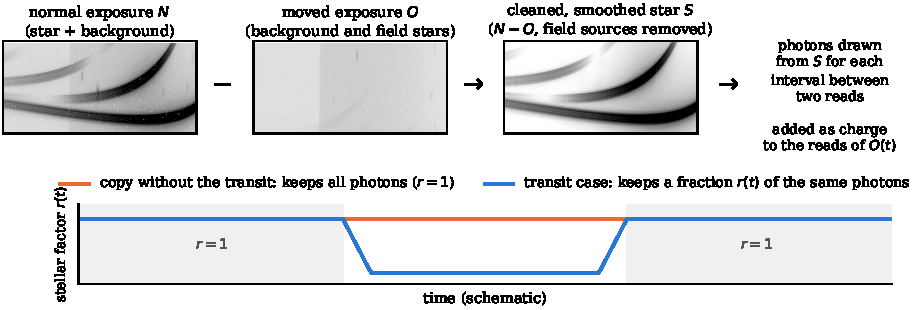
\includegraphics[width=\textwidth]{figures/pid4476_construction.pdf}
  \caption{Construction of the benchmark data. One set of photon
  arrivals is drawn from the cleaned image of the star for successive time
  intervals, accumulated into reads in the linear domain of the detector and
  added to the reads of the moved exposure, which is the same for both cases.
  The twin keeps all arrivals and the transit case keeps a fraction $r(t)$ of
  the same arrivals, so the two are identical on every integration that has
  lost no light to the transit since its reset. The lower panel shows the
  stellar factor $r(t)$, not the total flux, which also contains light that
  does not transit. The injected light curve is known exactly, whilst the
  fidelity of the image to the physical star is a separate question. Field
  sources in the moved exposure stay there and do not transit. The light curve
  is schematic.}
  \label{fig:4476-construction}
\end{figure*}

\begin{figure*}[t]
  \centering
  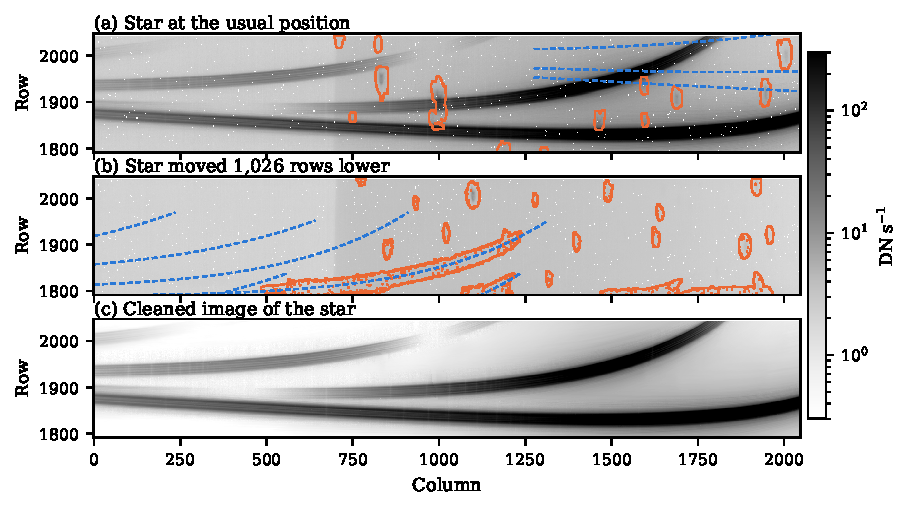
\includegraphics[width=0.92\textwidth]{figures/pid4476_star_and_carrier.pdf}
  \caption{The SOSS strip in programme 4476. (a) The exposure with the star at
  its usual position. (b) The exposure with the star moved 1,026 rows lower,
  into which the star is injected. (c) The cleaned image of the star, given by
  the difference between (a) and (b) with the field sources removed and the
  far wings smoothed (a preliminary version, made before the corrections for
  the sky and the halo of the moved star). Orange outlines mark the field
  sources found in each exposure. Blue dashed lines are traces of Gaia DR3
  stars with $G\leq20.5$, predicted with an empirical mapping from WASP-17,
  with the moved pointing aligned to the measured displacement of the
  target. The grey scale is logarithmic.}
  \label{fig:4476}
\end{figure*}

\subsection{Cleaning the image of the star}
\label{sec:cleaning-star}

The first problem is the field sources (Figure~\ref{fig:4476}). Because the
field moved with the telescope, the difference contains the field sources of
the first pointing as positive sources, which would transit together with the
target, and those of the second pointing as negative ones. I located them in
each exposure separately. The 13 sources of the first pointing were replaced in
$S$ by the profile of the star in neighbouring columns. For the 18 sources of
the second pointing, $S$ uses a local estimate of the background instead of
the second exposure, so that their light is not subtracted from the star. They
remain in $O(t)$ as real light that does not transit, as in any real
observation. The largest is the spectrum of a field star crossing order~1
between columns 484 and 1238, with up to 0.77\% of the light in a column. At
$1.874$ to $1.893\,\mu\mathrm{m}$, it would dilute a 1.5\% transit by 96~ppm
in a 40-row extraction box with ideal sky subtraction, and the pipelines must
handle it as they would in real data.

This source is consistent with the second order of a star with $G=17.7$ in
the Gaia catalogue \citep{GaiaDR3}: over the 26 columns checked, its median
separation from the predicted trace is 1.8 detector rows. The 13 compact
sources of the first pointing could not be matched securely to Gaia stars, so
their nature is unknown. Field stars lying exactly under the traces of the
target move with it, and these two exposures cannot separate them. Their
light stays in $S$ and becomes part of the injected star, so it does not
change the injected light curve. Near the
trace cores, the measured image differs from a smooth profile built from
neighbouring columns with a scatter of 2.4 to 2.9\% per pixel, and this
comparison found no further compact source beyond those removed.

The second problem is the faint wings. After the subtraction, the light of
the star is measured well into its wings, where it is comparable to or fainter
than the background (Figure~\ref{fig:4476-profiles}). With only ten
integrations in the first exposure, however, these wings are noisy. The
signal-to-noise ratio per pixel is 112 to 675 in the cores of the traces, but
only 2 to 3 at 40 to 200 rows from order~1 in the red. Beyond 40 rows from the
nearest trace, I therefore replaced the pixels by a running median along the
trace over 61 columns, blended with the data between 30 and 40 rows. On
average, this model differs from the measured pixels by about 0.16\% at 40 to
100 rows. Near the traces, $S$ keeps the measured image with its noise, which
becomes part of the injected star in the same way.

\begin{figure*}[t]
  \centering
  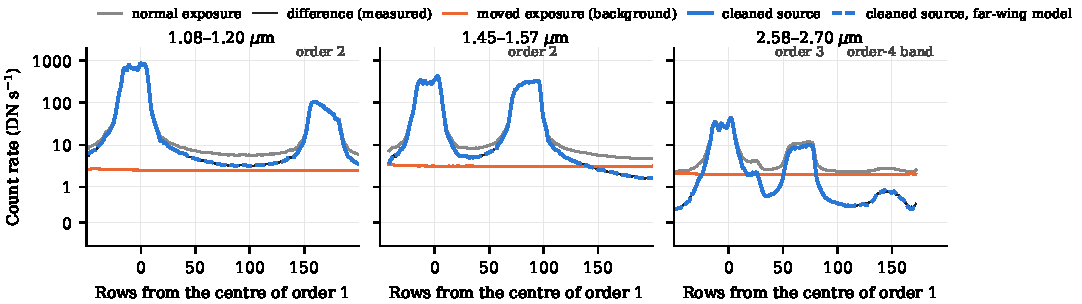
\includegraphics[width=\textwidth]{figures/pid4476_profiles.pdf}
  \caption{Median profiles across the trace of order 1 in three wavelength
  bands: the exposure with the star at its usual position (grey), the moved
  exposure, which provides the background at the same pixels (orange), their
  measured difference (black), and the cleaned image of the star (blue;
  dashed where the far-wing model is used, which depends on the distance from
  the nearest trace). The further peaks are order 2 in the left and middle
  panels, and order 3 and a faint band that is probably order 4 in the right
  panel. The vertical scale is linear near zero and logarithmic above, so that
  negative values are kept. The cleaned image is a preliminary version, made
  before the corrections for the sky and the halo of the moved star.}
  \label{fig:4476-profiles}
\end{figure*}

\subsection{Tests before any pipeline is scored}
\label{sec:tests}

Before any pipeline is run, the injected data must pass three tests. Firstly,
injecting nothing must return the calibrated ramps and count rates of the
moved exposure unchanged. Secondly, each case and its twin must be identical
in every integration that has lost no light to the transit since its reset.
Finally, the noise added with the star must follow photon statistics.

I then plan to score each method at two levels. At the first level, I
subtract the light that each method assigns to the star in the transit case
from that in its twin, and fit the size of the known injected loss of light. The shape of
the light curve is fixed, so neither the transit geometry nor the limb
darkening is fitted. The second level is the spectrum from
each pipeline's own transit fit. A pipeline that fails to recover the injected
transit is itself a result.

\subsection{Limitations}
\label{sec:benchmark-limits}

Even if the data pass these tests, the measured errors apply only to the star
and detector conditions of this benchmark, which has clear limitations.

Firstly, the star and its field differ from those of WASP-17. The star is brighter and the
sky fainter, at about 2.9~DN\,s$^{-1}$ per pixel compared with 4 to
6~DN\,s$^{-1}$ for WASP-17, so background light dilutes the transit less than
in the WASP-17 data. Because the star is of A type, its second and third
orders are also brighter relative to the first, which changes the overlap of
the orders that the pipelines must handle.

Secondly, the readout differs from that of a SOSS time series. The exposures are full frames read through
four outputs with 10.7~s frames, whereas SOSS time series read one output with
5.5~s frames. The strip is cut from these full frames but labelled as a SOSS
subarray, so a pipeline would by default subtract the bias of the subarray
readout. Every pipeline therefore receives the bias reference of the full-frame
readout, the only reference file that differs from its native choice. After
the strip's own reference-pixel correction, the variance of the noise per read
is 6 to 9\% higher than in the SOSS subarray. The $1/f$ noise per read is
4.92~DN, compared with 4.81~DN for WASP-17. An integration has at most five
groups, against eight for WASP-17, and integrations follow each other every
64~s rather than 49~s. At five groups the brightest pixels reach 89\% of
saturation. The saturation rule of one pipeline then newly flags 27\% of the
star's light in the extraction box, and the transit changes the flags on
2.3\% of it. I therefore also build versions with the first four groups, where
4.5\% is newly flagged and the transit changes the flags on 0.8\%, and with
the first three, where 0.26\% is newly flagged, almost all of it beside known
bad pixels. With three groups, the transit changes no flags in a typical
integration and at most 0.06\% of the light in any.

Thirdly, some effects are absent by construction. The injected star does not
move, so the small motions and shape changes of a real trace are missing. The
construction also omits any electronic response to the injected change in
illumination. The added photons are drawn independently in each pixel, so
their noise lacks the coupling between neighbouring pixels that a real
detector introduces. The real noise already present in the moved exposure is
kept.

I also compared the shapes of the injected and observed ramps. Because the
star is added before the detector's nonlinearity is applied
(Section~\ref{sec:measuring-star}), the injected ramps of the brightest pixels
curve over at high fill as real ramps do. For pixels
grouped by brightness, the median changes between consecutive reads agree
with those of the exposure with the star at its usual position to within 1\%
above 300~DN\,s$^{-1}$, although the
median injected ramp lies about 140 to 230~DN above the real one. In the two
faintest groups, below 30~DN\,s$^{-1}$, the median changes between reads
differ by up to 8\%, which remains a limitation.

The injected transit also fixes the limb darkening against which every
pipeline is tested. This is one quadratic law computed from PHOENIX models over
a declared passband, which none of the pipelines uses natively. The star is
also hotter than the limb-darkening grid from which two of the pipelines take
their reference, so their own fits carry a known mismatch. The first scoring
level avoids a fitted limb-darkening prior, although its result can still
depend on the injected light curve. In a control, every pipeline will use the
injected coefficients in both its white-light and spectral fits, and each
native setup will state how it treats a star outside its grid. The injected
limb darkening is therefore a stated challenge for the pipelines.

These limitations restrict what the benchmark can show, but they leave the
injected light curve unchanged. The six science visits have no independently
measured image of the star, so the benchmark cannot be repeated on them, and
they will be analysed as real data (Section~\ref{sec:plan}).
